\documentclass[11pt]{article}

\usepackage[
top    = 2.50cm,% presumably you don't want it to be 0pt as well?
bottom = 2.50cm,
left   = 2cm,
right  = 2cm,
marginparsep = 0pt,
marginparwidth=0pt,
]{geometry}
\usepackage{amssymb}
\usepackage{fancyhdr}
\usepackage[most]{tcolorbox}
\usepackage{siunitx}
\usepackage{amsmath}
\usepackage{tikz}
\usepackage{graphicx}
\usetikzlibrary{decorations.markings}
\usepackage{caption}
\usepackage{pgfplots}
\usepackage{multicol}
\pagestyle{fancy}
\fancyhead[l]{Electromagnetism - Abridged edition}
\fancyhead[r]{Giorgio Grigolo {\textcopyright}}
\tikzset{
	mypath/.style={
		postaction=decorate,
		decoration={markings,
			mark=at position #1 with {\coordinate (x);\arrow{>}}},
		thick},
	>=stealth
}
\begin{document}                          
\section{Magnetic fields: }
\subsection{Total flux equation: }
\begin{equation}
	\phi = \mathrm{B}A\tag{\si\weber}
\end{equation}


  \section{Tesla}
  \begin{center}
  	\textit{The flux density of the field that exerts a force of 1\si{\newton} on a 1\si{\meter} long wire, placed at right angles to the field and carrying a current of 1\si{\ampere}.}
  \end{center}
\begin{equation}
	F=BIl\tag{\si{\tesla}}
\end{equation}
\begin{center}
	Where $B$ is the component of the field that is \textbf{perpendicular} to the current, $I$ the \textbf{current} (\si\ampere) in the system and $l$ the \textbf{length} (\si\meter).
\end{center}
\section{Lorentz Force: }
\begin{equation}
	F=Bqv\tag{\si{\newton}}
\end{equation}
\begin{center}
	Where $F$ is the force on a moving charge in a magnetic field, $B$ is the \textbf{total flux} (\si\weber) in the magnetic field, $q$ is the \textbf{charge} (\si{\coulomb}) of the moving particle and $v$ its \textbf{velocity} (\si{\meter\per\second}).
\end{center}

\section{The Laws of Electromagnetic Induction: }

\subsection{Faraday's Law}

\begin{center}
	\textit{An e.m.f. is induced in a conductor whenever the magnetic flux taht links with that conductor changes. The size of the e.m.f. is equal to the rate of change of the flux linkage.}
\end{center}

\subsection{Lenz's Law}

\begin{center}
	\textit{The direction of the induced e.m.f./current is always such as to oppose the change causing it.}
\end{center}

\subsection{Equation: }

\begin{equation}
	E = \frac{\Delta N \phi}{\Delta t}\tag{\si\volt}
\end{equation}
\begin{center}
	Where $E$ is the \textbf{induced e.m.f.} (\si{\volt}), the product $N\phi$ is the \textbf{flux linkage} (\si\weber), $N$ is the number of turns of the coil and  $\phi$ is the \textbf{magnetic flux} (\si{\weber}).
\end{center}
\subsection{Conductor Cutting Lines of Flux: }
\begin{equation}
	E=Blv\tag{\si\volt}
\end{equation}
\begin{center}
	Where $E$ is the induced e.m.f. $l$ is the length of the conductor cutting the field and $v$ is the speed at which the conductor cuts the field.
\end{center}

\section{A.C. Generation: }
\subsection{Rotating rectangular coil: }
\subsubsection{Diagram : }

\begin{center}
	\includegraphics[width=0.5\linewidth]{"pictures/coi"}
\end{center} 

\begin{multicols}{2}
	\begin{center}
		perpendicular $\implies$ peak e.m.f.
	\end{center}
	\begin{center}
		parallel $\implies$ no e.m.f.
	\end{center}
\end{multicols}

\subsubsection{Induced e.m.f. formula: }
\begin{equation}
	E=2\pi f\cdot BAN \cdot\sin(2\pi f t)\tag{\si{\volt}}
\end{equation}

\subsubsection{Peak induced e.m.f formula: }
\begin{equation}
	E_0 = 2\pi fBAN\tag{\si\volt}
\end{equation}
\section{R.M.S. value of an A.C. current: }
\begin{equation}
	I_{RMS} = \frac{I_0}{\sqrt2}
\end{equation}
\end{document}
\begin{center}
	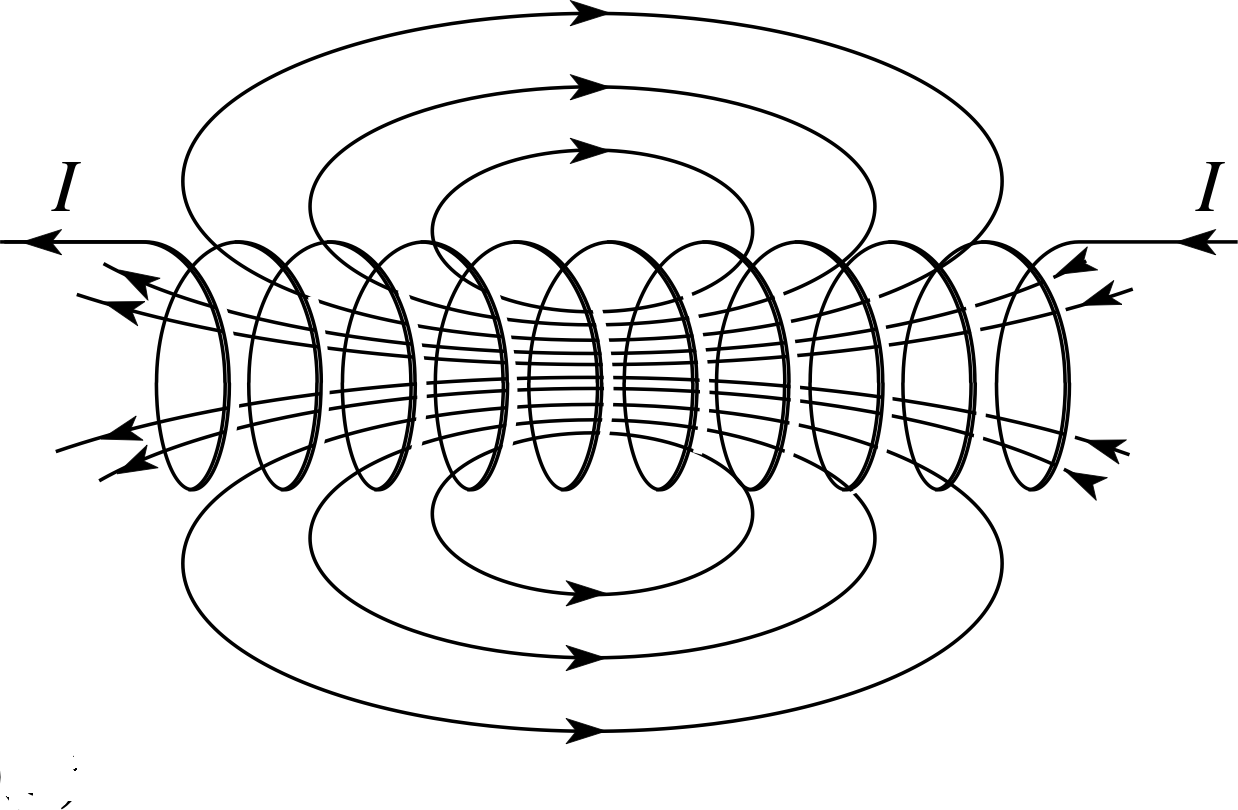
\includegraphics[width=0.5\linewidth]{pictures/solenoid}
\end{center}